\documentclass[10pt,a4paper]{article}
\usepackage[utf8]{inputenc}
\usepackage[ngerman]{babel}
\usepackage{amsmath, amsfonts, amssymb}

\usepackage[left=3.5cm,right=3.5cm, bottom=3cm, top=3cm]{geometry}

\usepackage{setspace}				% für Zeilenabstand
\usepackage[pdftex]{graphicx}	% zum Einbinden von Grafiken

\usepackage[skip=10pt]{caption} % Erhöht den Abstand zwischen Überschriften und Grafiken

\usepackage	[colorlinks,
			linkcolor=black,
			citecolor= black,
			urlcolor = blue, 
			bookmarksopen=true,
			bookmarksnumbered=true,
			pdfusetitle]{hyperref}				% erzeugt Hyperlinks im Inhaltsverzeichnis

\usepackage{natbib}								% Zitierweise
\bibliographystyle{chicago}

\begin{document}
\author{Björn Bos\thanks{bjoern.bos@web.de}}
\title{Nächster Halt: Armutsviertel? Eine Bahnfahrt mit der U3 durch Hamburg}
\date{Mai 2019}

\maketitle

\doublespacing

\section*{Motivation}
In Hamburg findet man in vielen Straßen prunkvolle Fassaden und Villen reihen sich an Alster und Elbe nebeneinander. Doch ist Hamburg damit reich? Und partizipieren alle Hamburger im gleichen Maß vom allgemein angenommen Wohlstand?

So sehr das Wasser und der Hafen den Wohlstand der Stadt bedingt hat, so sehr stellt es auch unsichtbare Trennwand dar, die die Stadt in ärmere und reichere Gebiete einteilt. Während die Stadtteile nördlich der Elbe durchschnittlich reicher sind, geht es südlich der Elbe bescheidener und deutlich ärmer einher. Aber auch wenn man sich die Stadtgebiete um die Alster anschaut, wird man Ungleichheiten feststellen.

Um auf solche regionalen Ungleichheiten aufmerksam zu machen, zeichnet dieser Essay eine Fahrt mit der Stadtbahn U3 nach, deren Verlauf einmal um die ganze Alster führt. Auf gut 20km führt sie durch verschiedenste Stadtgebiete und hält an 25 unterschiedlichen Stationen. Sie beginnt in Wandsbek-Gartenstadt, führt im Osten über Barmbek und Berliner Tor zum Hauptbahnhof, an der Elbe über Baumwall und Landungsbrücken nach St. Pauli, bevor sie im Westen über den Eppendorfer Baum zurück nach Wandsbek-Gartenstadt führt.

Dieser Essay analysiert sozial-ökonomische Indikatoren der Stadtgebiete, die sich in unmittelbarer Nähe zu diesen Haltestellen befinden. Er gibt damit einen Eindruck welche Menschen man im Umkreis um eben jene Haltestellen trifft. Dieser Essay greift damit die Idee von \citet{New_Yorker} und \citet{M29} auf, welche ähnliche Analysen für die New Yorker U-Bahnlinien und die Buslinie M26 in Berlin veröffentlicht haben.

Dieser Essay verdeutlicht, wie nah Arm und Reich sich in Hamburg sein können. Er zeigt wie stark soziale und wirtschaftliche Indikatoren auf einer Strecke von nur 20km schwanken können und an welchen Haltestellen man welche Menschen am ehesten trifft.


\section*{Daten und Methodik}
Grundlage dieses Essays sind Daten des Sozialmonitoring-Bericht \citep{Sozialmonitoring_Bericht_2018}. Für 941 kleinteilige Statistische Gebiete wurden dafür Angaben zur sozialräumlichen Entwicklung zusammengetragen. Darin enthalten sind beispielsweise Daten zur Arbeitslosigkeit, zu Schulabschlüssen und zur Mindestsicherung unter Kindern und Rentnern. Die Koordinaten der Haltestellen der U3 sowie deren Linienverlauf wurden aus GTFS Daten des Hamburger Verkehrsverbund abgeleitet. Schließlich wurden ebenso die Ergebnisse der Zweitstimmen der Bundestagswahl 2017 pro Wahlbezirk berücksichtigt. Alle diese Daten sind öffentlich verfügbar und für nicht-kommerzielle Zwecke nutzbar.

Abbildung~\ref{fig:map} zeigt eine Karte der Statistischen Gebiete die einen Radius von 300m um eine Haltestelle der U3 schneiden. Damit werden nur jene Quartiere berücksichtigt werden, deren Bewohner die einzelnen Haltestellen morgens am ehesten aufsuchen und abends am ehestens verlassen.

\begin{figure}[h!]
	\centering
	\caption{Berücksichtigte Statistische Gebiete Hamburgs, sowie die Haltestellen und der Linienverlauf der U3.}
	\label{fig:map}
	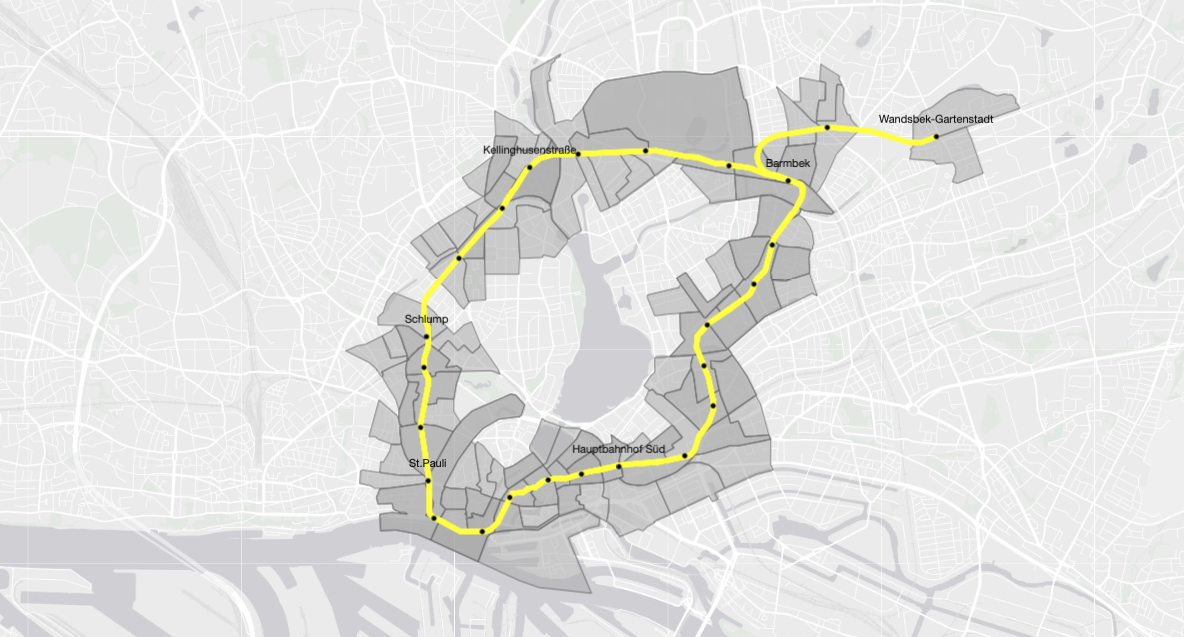
\includegraphics[width=0.7\linewidth]{../../02_results/map}
\end{figure}

Für die Gebiete um eine Haltestelle wurden anschließend die Mittelwerte ausgewählter sozial-ökonomischer Indikatoren berechnet. Einzige Ausnahme bilden die Haltestellen Mön-ckebergstraße und Rathaus. Da in deren Umgebung weniger als 400 Personen wohnen, wurden die sozial-ökonomischen Indikatoren für diese Gebiete nicht berücksichtigt. Ebenso wurde ein Statistisches Gebiete südlich der Elbe nicht berücksichtigt, welches streng genommen einen Radius von 300m um die Station Landungsbrücken schneiden.


\section*{Arbeitslosigkeit und Altersarmut}
Entlang der U3 gibt es starke Schwankungen in der Arbeitslosigkeit wie Abbildung~\ref{fig:unemployment} zeigt. Während sie zwischen Barmek und Berliner Tor nur gering zwischen 4,1\% und 4,7\% schwankt, können wir sehr hohe Werte von mehr als 7\% in den Gebieten um den Hauptbahnhof, St. Pauli und der Feldstraße beobachten. Im weiteren Verlauf sinkt sie allerdings rapide und fällt auf Werte von unter 2\% beim Eppendorfer Baum.

\begin{figure}[h!]
	\centering
	\caption{Anteil der Arbeitslosen unter der Erwerbsbevölkerung.}
	\label{fig:unemployment}
	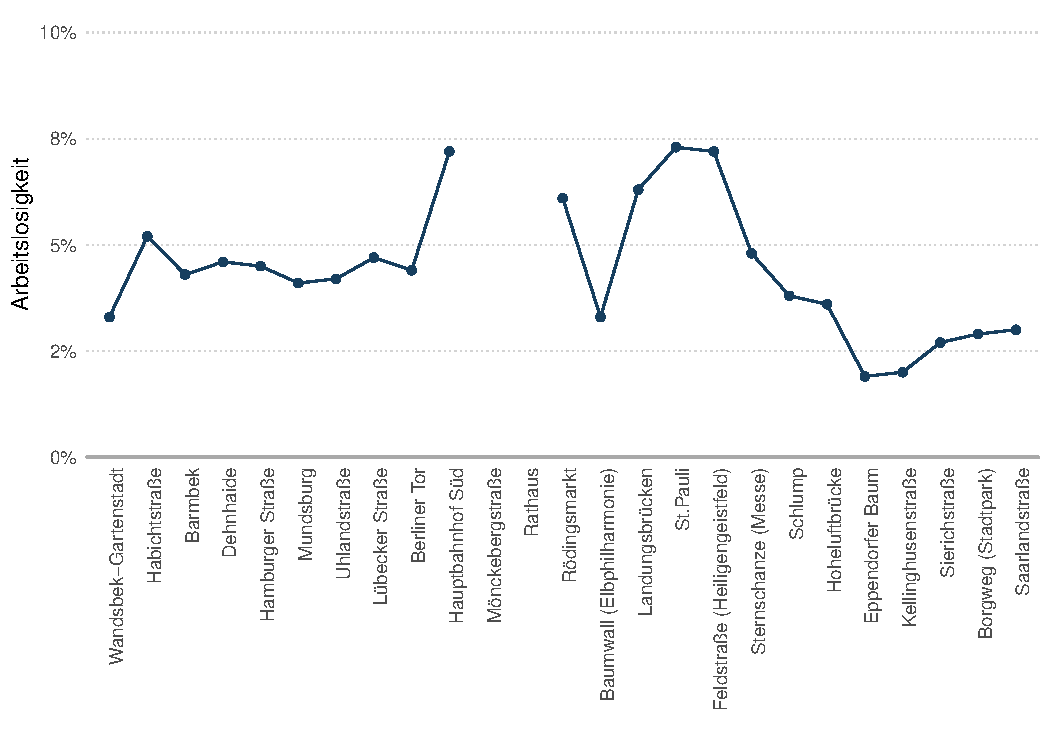
\includegraphics[width=0.8\linewidth]{../../02_results/fig_unemployment.pdf}
\end{figure}

Ähnliches können wir in Hinblick auf die Altersarmut beobachten. Abbildung~\ref{fig:mindestsicherung_alter} zeigt den Anteil der Empfänger*Innen von Mindestsicherung im Alter. Auch hier sehen wir ein ähnliches Muster und stellen fest, dass besonders im Bereich der Hauptbahnhofs, St. Pauli und der Feldstraße mehr als jede fünfte Person über 65 Jahren Mindestsicherung erhält und vom Risiko der Altersarmut betroffen ist.

\begin{figure}[h!]
	\centering
	\caption{Anteil der Personen über 65 Jahren mit Mindestsicherung.}
	\label{fig:mindestsicherung_alter}
	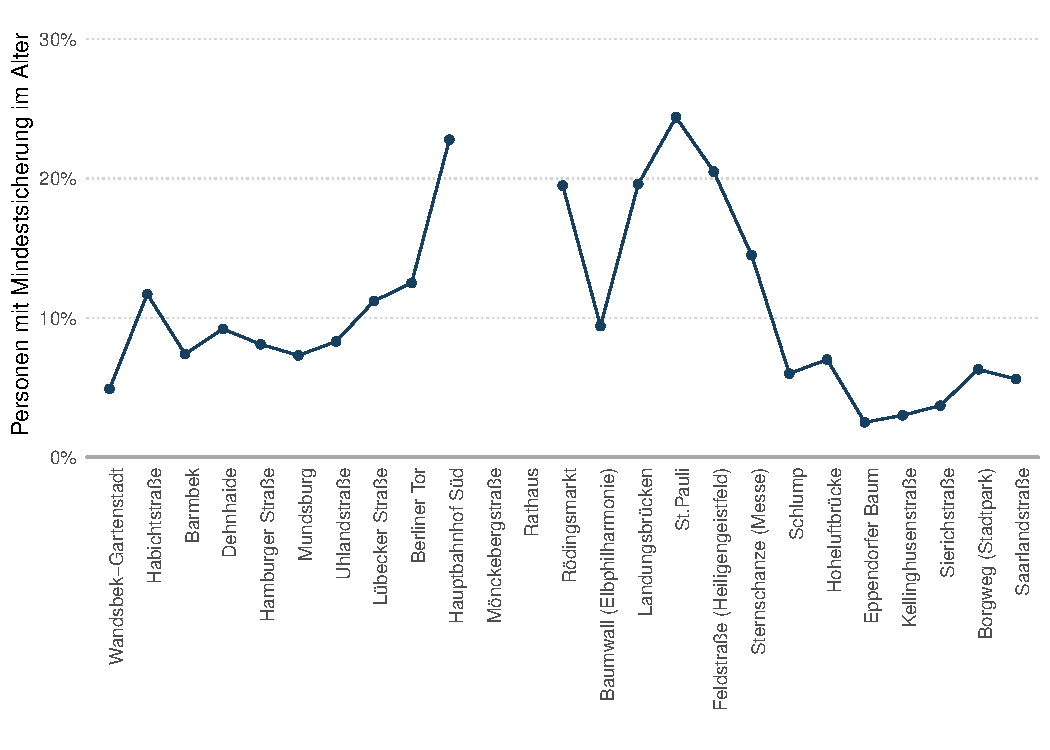
\includegraphics[width=0.8\linewidth]{../../02_results/fig_mindestsicherung_alter.pdf}
\end{figure}


\section*{Chancengleichheit unter Kindern und Jugendlichen}
Um später nicht in Arbeitslosigkeit oder Armut zu geraten, kann Bildung ein entscheidender Faktor sein. Doch wie sieht es aus mit der Chancengleichheit unter Kindern und Jugendlichen? Wie sind die Chancen verteilt, dass Schulabgänger studieren können? Ein Blick auf den Anteil der Schüler die \textit{kein} Abitur haben, verrät uns mehr darüber.

Abbildung~\ref{fig:schulabgaenger_ohne_abitur} zeigt, dass östlich der Alster 29\% bis 54\% der Schulabgänger kein Abitur haben. Analog zur Arbeitslosigkeit und Altersarmut hat die Mehrheit der Schüler im Bereich zwischen den Landungsbrücken und der Feldstraße ebenso kein Abitur und kann damit nicht direkt an einer Universität studieren. Nach der Feldstraße hingegen ist die Chance Abiturienten in der U3 zu treffen signifikant höher. Besonders beim Eppendorfer Baum und der Kellinghusenstraßen verlässt nur knapp 10~Prozent der Schüler die Schule \textit{ohne} Abitur.

\begin{figure}[h!]
	\centering
	\caption{Anteil der Schulabgänger \textit{ohne} Abitur.}
	\label{fig:schulabgaenger_ohne_abitur}
	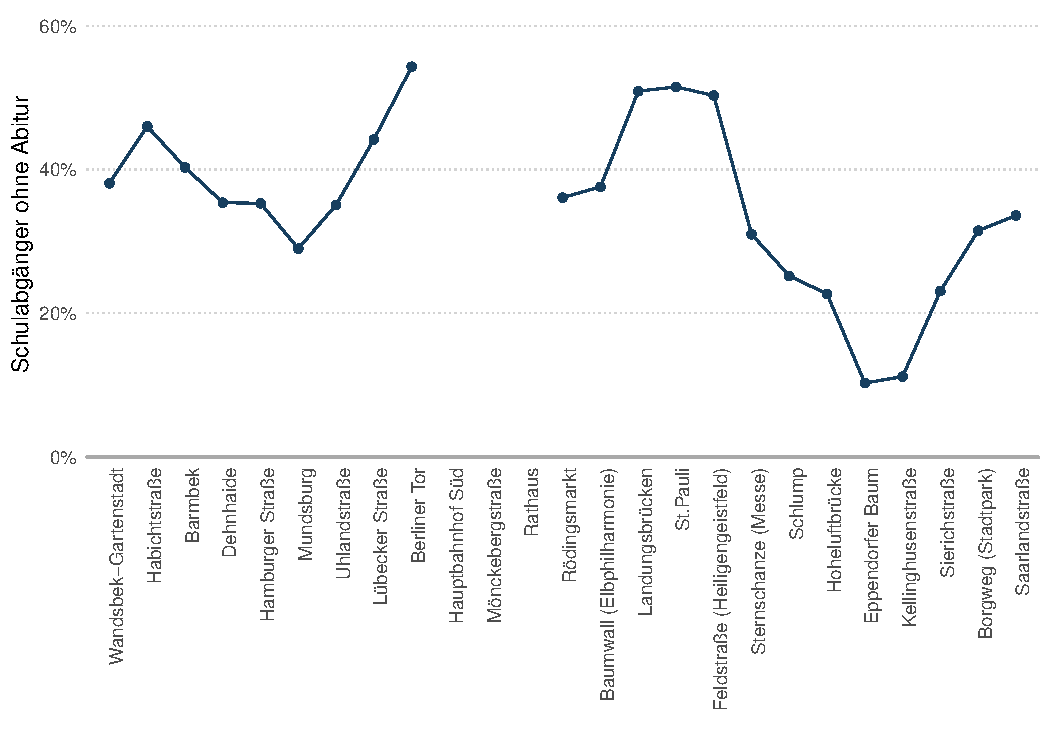
\includegraphics[width=0.8\linewidth]{../../02_results/fig_schulabgaenger_ohne_abitur.pdf}
\end{figure}


\section*{Parteipräferenzen}
Und schließlich können uns die Wahlergebnisse der letzten Bundestagswahl in 2017 einen Eindruck geben, welche Themen und Standpunkte den Personen entlang der U3 wichtig sind. Abbildung~\ref{fig:ergebnis_bundestagswahl_2017} zeigt dazu den Anteil der Zeitstimmen für die beiden größten Parteien SPD und CDU.

Auch hier ist erkennbar, dass sich das Wahlverhalten von Halstestelle zu Haltestelle ändern kann. Obwohl der Abstand beider Parteien zueinander häufig nur gering ist, können wir einen besonders großen Vorsprung der CDU vor der SPD zwischen dem Eppendorfer Baum und der Sierichstraße beobachten.

\begin{figure}[h!]
	\centering
	\caption{Ergebnisse der SPD und CDU in der Bundestagswahl 2017.}
	\label{fig:ergebnis_bundestagswahl_2017}
	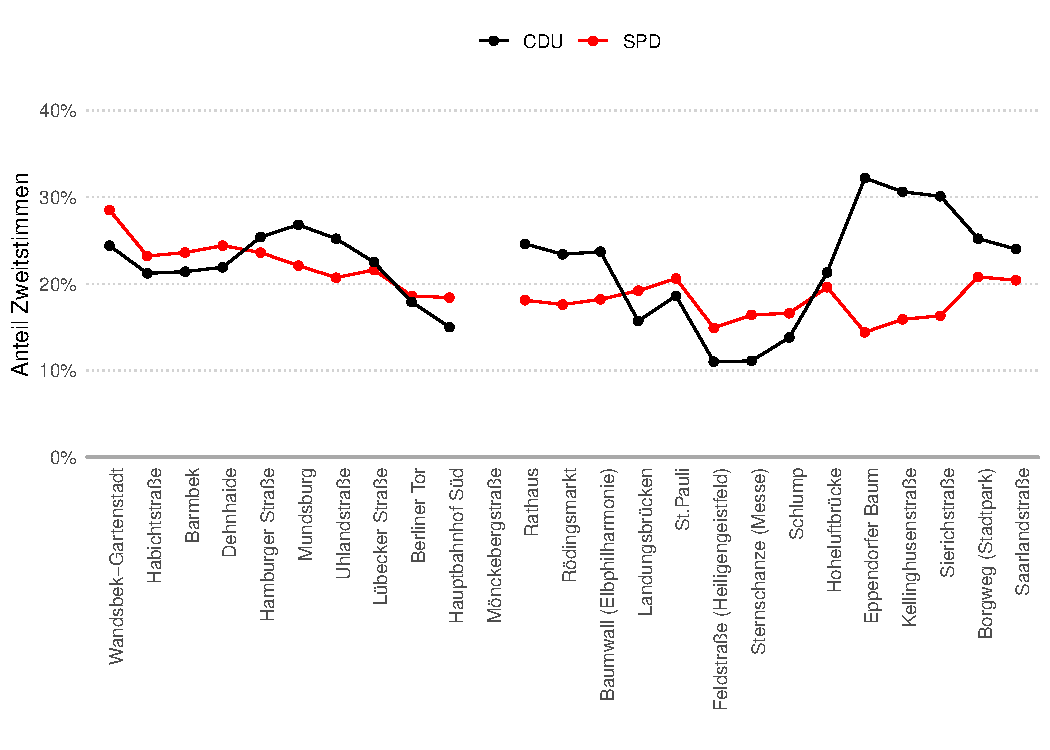
\includegraphics[width=0.8\linewidth]{../../02_results/fig_ergebnis_bundestagswahl_2017.pdf}
\end{figure}


\section*{Zusammenfassung}
Dieser Essay zeigt, dass Arm und Reich in Hamburg nicht weit voneinander entfernt sein müssen. Fährt man beispielsweise mit der U3 kommt man durch Gebiete in denen Arm und Reich häufig nur ein paar Haltestellen entfernt liegen.

Ganz besonders fällt dies auf wenn man zwischen den Landungsbrücken und der Kellinghusenstraße unterwegs ist.  Während im Gebiet an der Elbe eine hohe Arbeitslosigkeit und Altersarmut herrscht, sind diese nord-westlich der Alster fast kaum vorhanden. Ebenso machen dort deutlich mehr Schülerinnen und Schüler Abitur und haben bessere Chancen auf einen Studienplatz.


%==================================================================
%	References
%==================================================================

\onehalfspacing
\bibliography{../literature}

%==================================================================
%	Appendix
%==================================================================

\section*{Digitaler Anhang }
Ein digitaler Anhang ist unter \url{https://github.com/bjoernbos/beitrag_armes_hh_reiches_hh/} verfügbar. Über diesen Link sind der Code zum Download aller Daten, zur Datenaufbereitung und zur Reproduktion aller Grafiken und Karten. Ebenso können dieses PDF-Dokument und eine \href{http://bjoernbos.github.io/beitrag_armes_hh_reiches_hh/}{interaktive Version (HTML)} dieses Essays abgerufen werden.


\end{document}